\documentclass[tikz,border=5mm]{standalone}
\usepackage{tikz}

\begin{document}
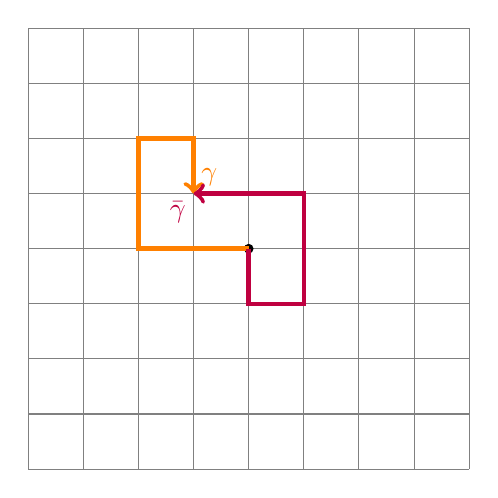
\begin{tikzpicture}[scale=0.7]
    % Draw an 8x8 grid, which has 9x9 vertices from (0,0) to (8,8)
    \draw[gray, thin] (0,0) grid (8,8);

    % Define the starting vertex at the true center
    \coordinate (start) at (4,4);
    \fill[black] (start) circle (2.5pt); % Mark the starting vertex

    % Path 1: LLUURD, labeled as \gamma
    % start -> (3,4) -> (2,4) -> (2,5) -> (2,6) -> (3,6) -> (3,5)
    \draw[orange, ultra thick, ->] (start)
        -- ++(-1,0) % L
        -- ++(-1,0) % L
        -- ++(0,1)  % U
        -- ++(0,1)  % U
        -- ++(1,0)  % R
        -- ++(0,-1) % D
        node[above right, inner sep=2pt] {$\gamma$};

    % Path 2: DRUULL, labeled as \bar{\gamma}
    % start -> (4,3) -> (5,3) -> (5,4) -> (5,5) -> (4,5) -> (3,5)
    \draw[purple, ultra thick, ->] (start)
        -- ++(0,-1) % D
        -- ++(1,0)  % R
        -- ++(0,1)  % U
        -- ++(0,1)  % U
        -- ++(-1,0) % L
        -- ++(-1,0) % L
        node[below left, inner sep=2pt] {$\bar{\gamma}$};
\end{tikzpicture}
\end{document}